% !TEX encoding = UTF-8
% !TEX TS-program = pdflatex
% !TEX root = ../Tesi.tex
% !TEX spellcheck = it-IT

%************************************************
\chapter{Introduzione allo logica dello spazio}
\label{cap:spazio}
%************************************************

\begin{flushright}{\slshape
  …sì, per cui una chiesa barocca ha sotto di sé, \\
  accessibile, una chiesa romanica, \\
  sotto la chiesa romanica una basilica paleocristiana, \\
  poi si scende ancora e c’è il mitreo romano… \\
  Questa è Roma. \\
  Però, invece, apparentemente Roma è appunto atemporale, \\
  sembra non offrire nulla; \\
  e gli accessi sono segreti, alla vera realtà di Roma. \\
  Quindi corrisponde assai bene allo stadio opaco dell’infanzia e dell’adolescenza, \\
  quando si è in preda a questa cosa strana che è il voler scrivere…} \\ \medskip
    --- G. Agamben
\end{flushright}


%\begin{figure}
%\centering
%\subfloat[Tetraedro inscritto in un cubo]
%{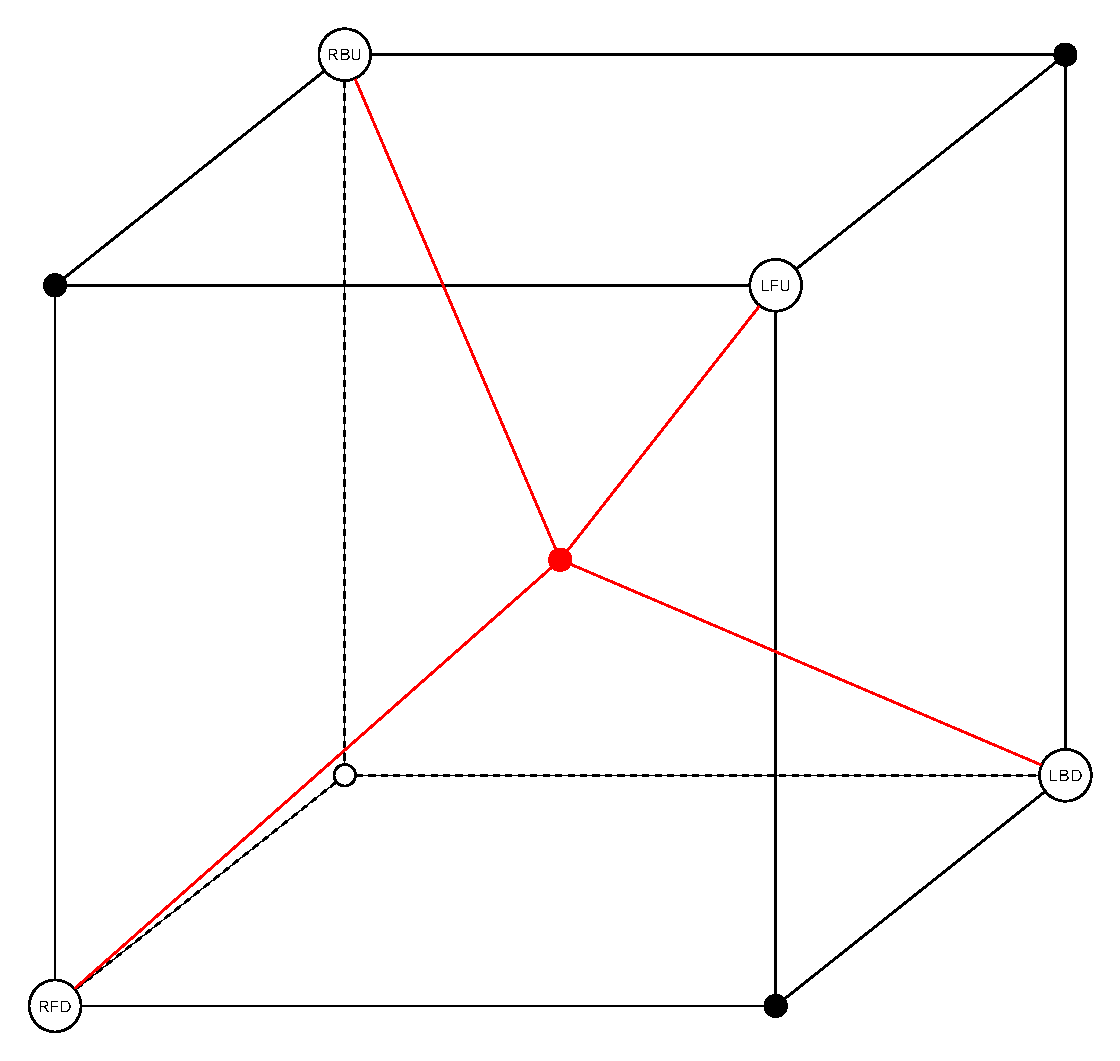
\includegraphics[width=.45\columnwidth]{tetrarec-cube}} \quad
%\subfloat[Spazio Tetraedrico]
%{\label{fig:tetracube}%
%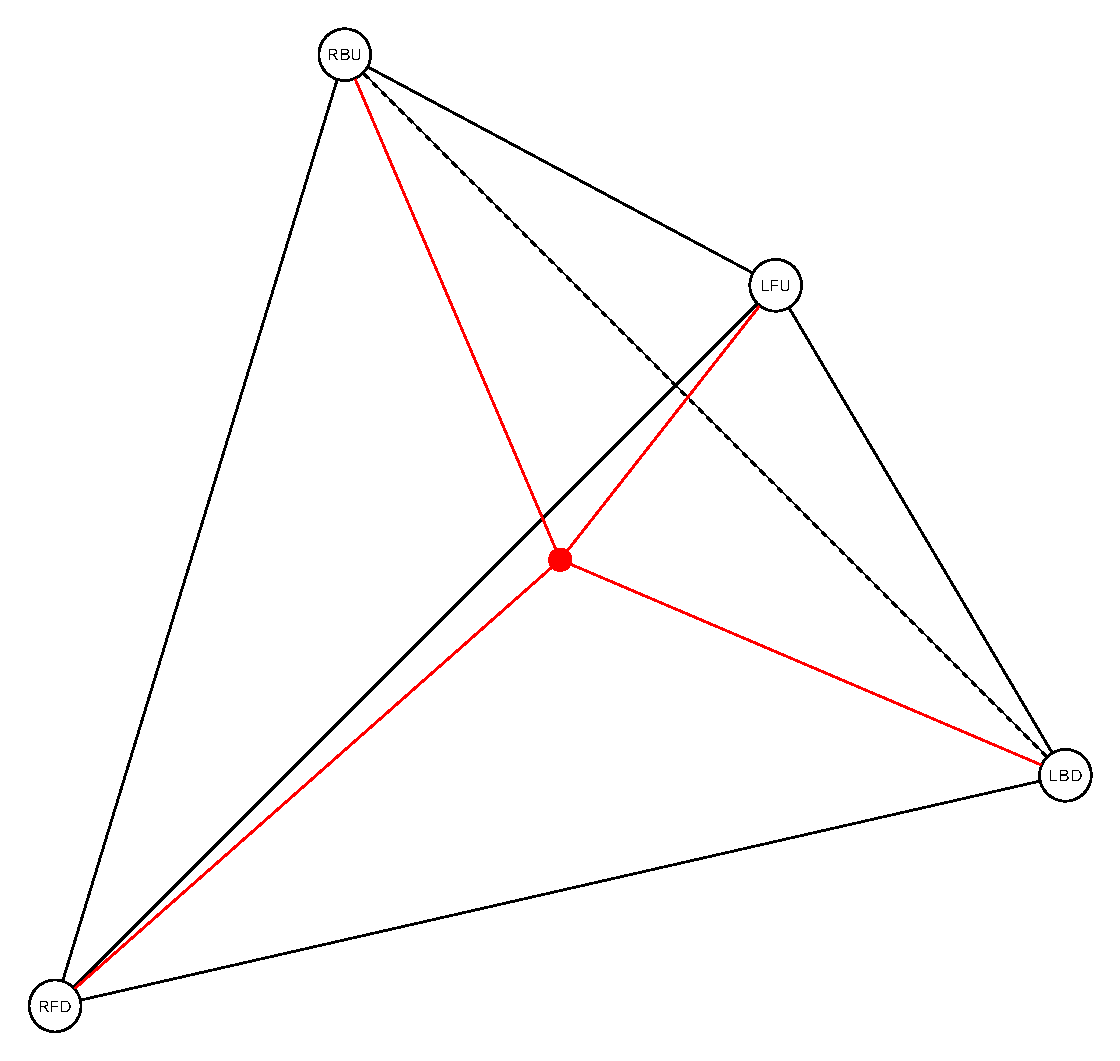
\includegraphics[width=.45\columnwidth]{tetrarec-tetrahedron}} \\
%\caption[Spazio Tetraedrico]{Spazio Tetraedrico}
%\label{fig:tetratetra}
%\end{figure}


%\begin{figure}
%\centering
%{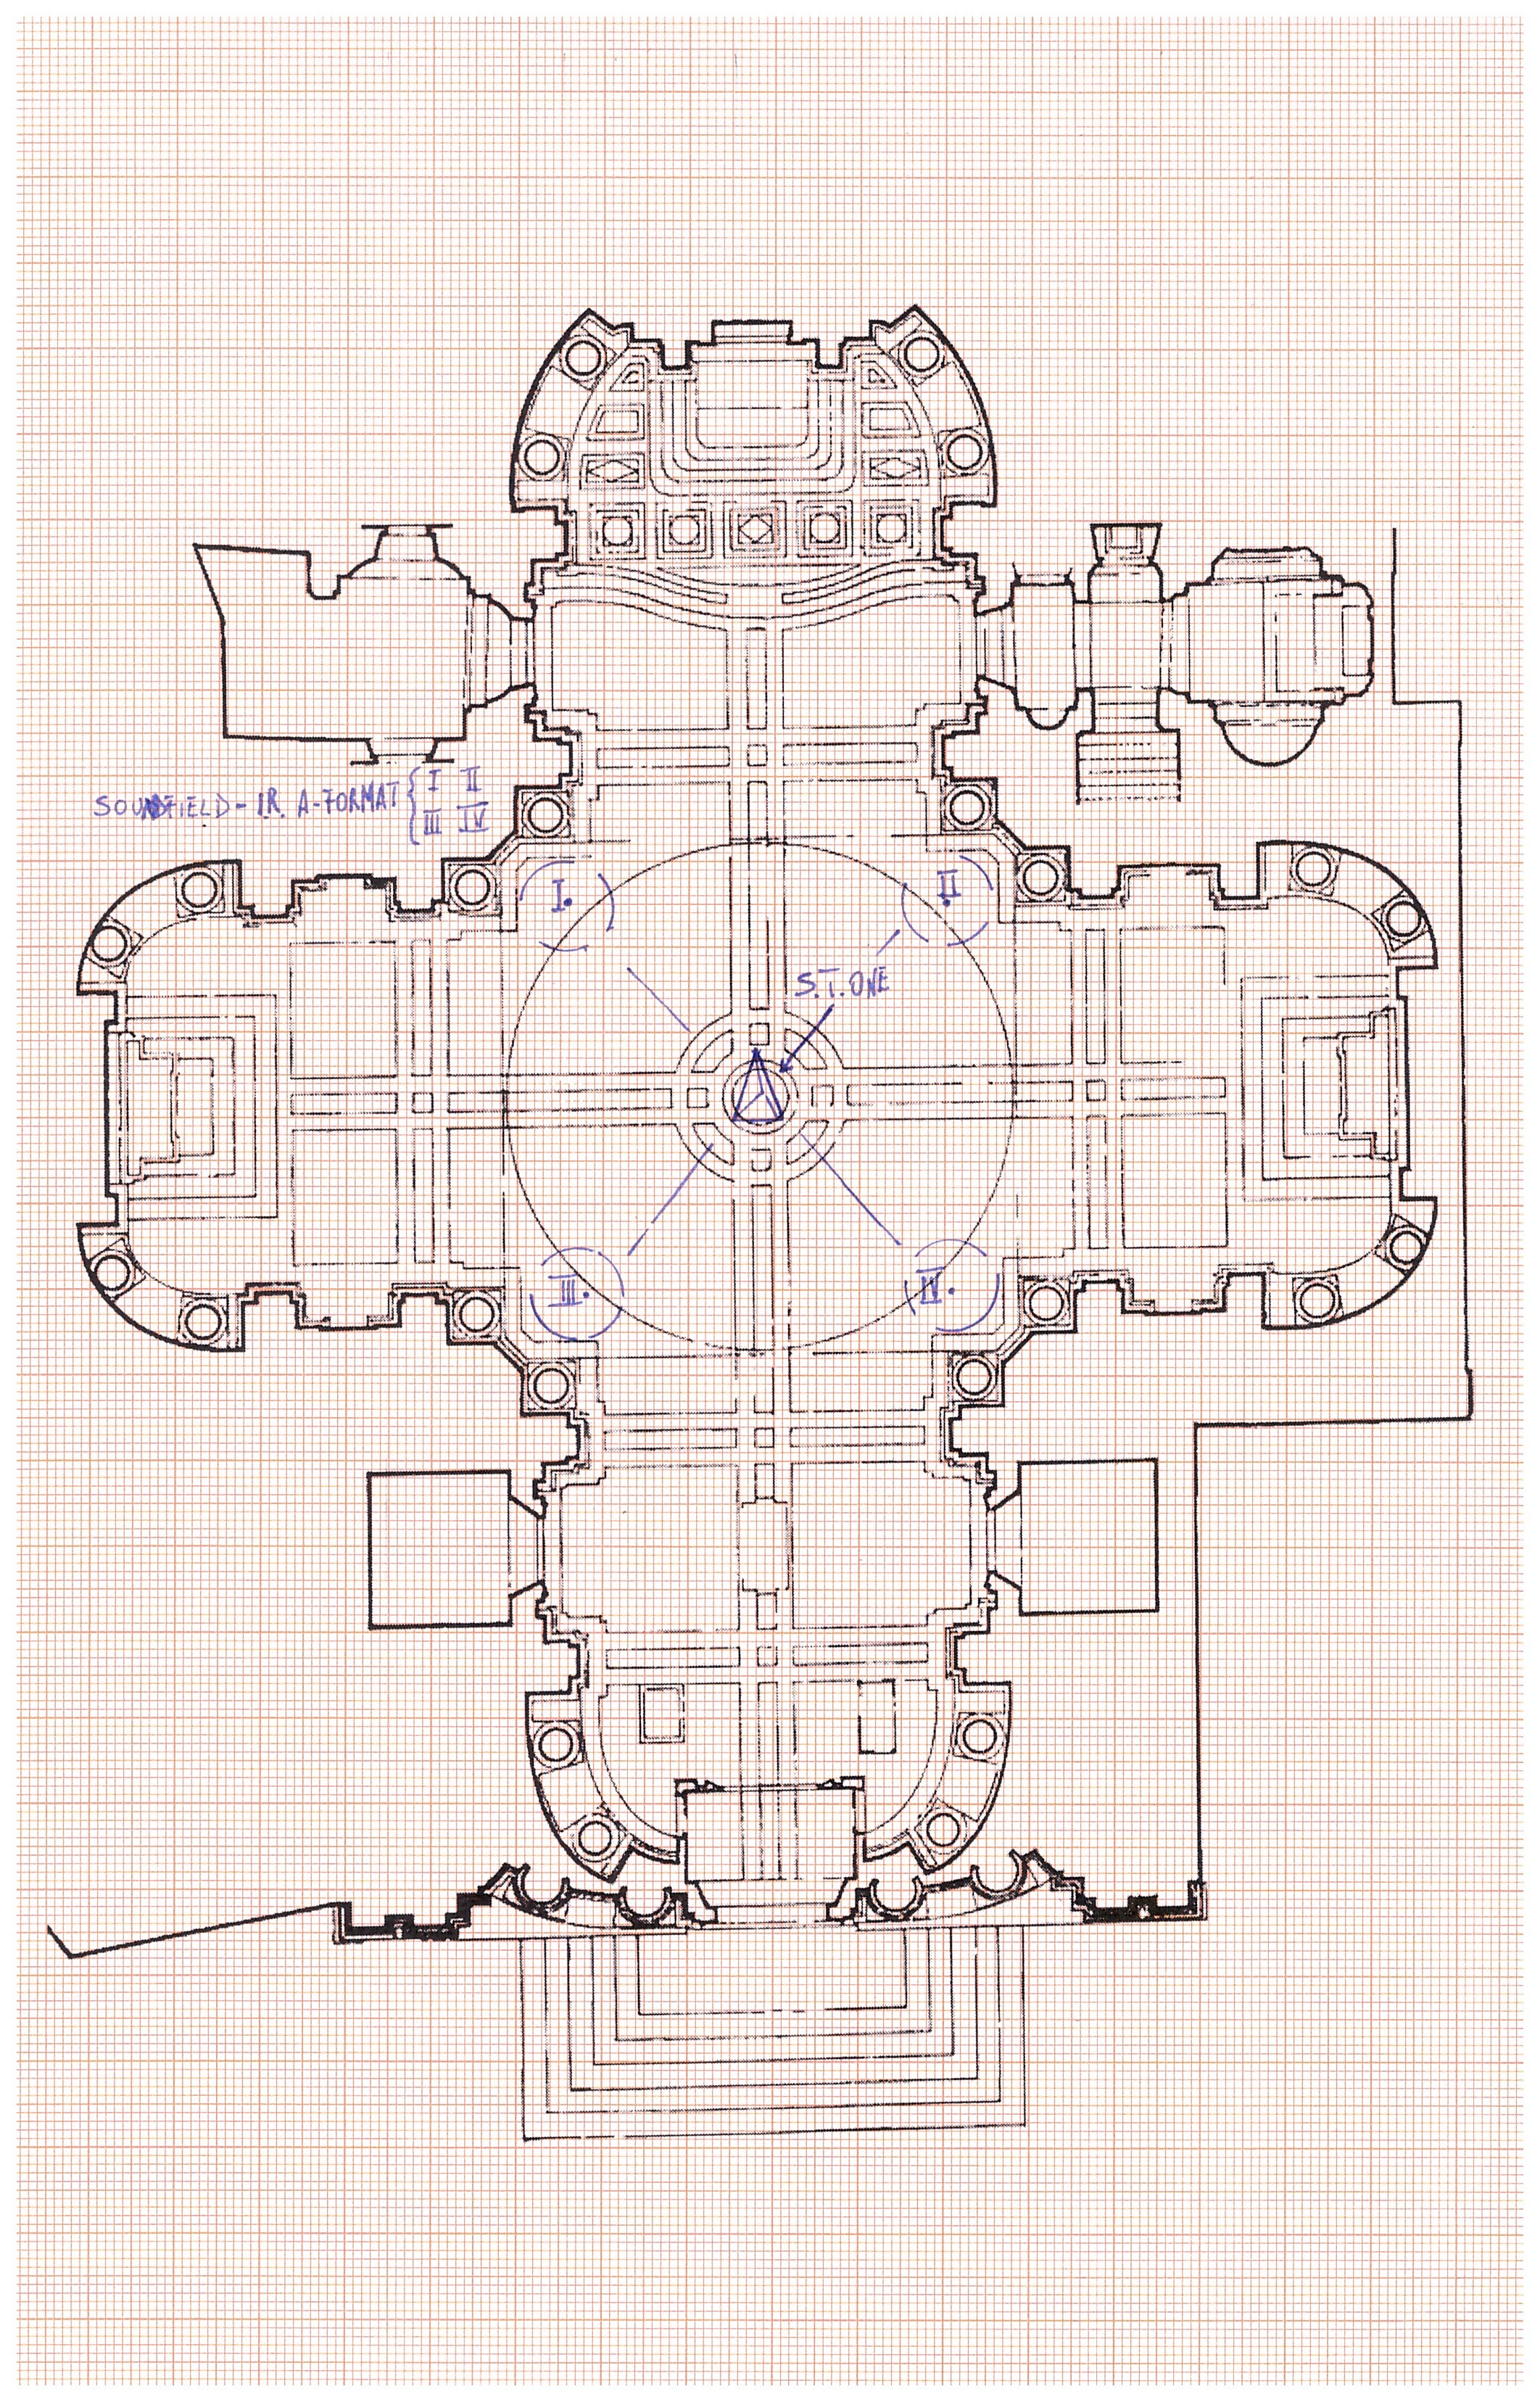
\includegraphics[width=.95\columnwidth]{Pianta_chiesa}}
%\caption[Pianta S. Luca]{Pianta S. Luca}
%\label{fig:tetratetra}
%\end{figure}

%discorso riverbero non come elaborazione dell'amplificazione ma come costruzione delle
%riflesioni ambientali. Le distanze hai 4 stone identisci cosi da dislocare gli altoparlanti
%facilmente. Posto simmetrico posto. Filmarmonica in

Nel descrivere il percorso di ricerca applicata allo spazio espressa in questa
tesi si può definire il duplice ruolo \emph{strutturale} del riverbero.

Riverbero \emph{struttura-architettonica} come definizione dell'ambiente,
custodia del rito e dell'idea musicale.

Riverbero \emph{struttura-musicale} come culla di risonanze cercate nella
scrittura e nei gesti, particelle del rito celato nel tubo sonoro e nel suo sconfinamento architettonico.

I riverberi architettonici, siano essi locali che generali, non acquisiscono funzione di elaborazione
di un suono amplificato. L'altoparlante non ha funzione di amplificazione ma di dimensionamento della forma
acustica della chiesa. C'è una dimensione spaziale di creazione, di sintesi e simbiosi acustica con lo strumento
che non assume mai funzione di elaborazione. La sola voce acustica dello strumento rischierebbe,
in un confronto con una diffusione elettroacustica convenzionale, di scindersi dalla sua immagine riflessa.

La riflessione, qualità intrinseca del riverbero, è oggetto di analisi e sintesi polidimensionale. 

La riflessione, per confrontarsi a pari caratteristiche con la voce acustica dello strumento musicale,
deve poter essere descritta nello spazio come un elemento polidimensionale tempovariabile.
Solo in questo modo ci si può permettere di collocare le due entità, ormai due voci dello
stesso canto, in due luoghi diversi della sala da concerto ed ottenerne un unico e solido
corpo sonoro, mosso e stazionario come nella chiesa. 

La scelta del sistema elettroacustico S.T.ONE è quindi parte attiva nella composizione,
elementi di dialogo strutturale e quindi al tempo stesso archiettonico e musicale.

La scelta del numero minimo di diffusori, quattro, si colloca tra i punti di equilibrio tra
minima definizione tridimensionale e resa acustica in regime di verosimiglianza.  

Lo stesso Michael Gerzon identifica in tre le sorgenti per la descrizine planare e q	uattro per la descizione perifonica.
Su questo principio si è operata una divisione dello spazio acustico descritto dalle mura in quattro regioni facilmente 
replicabili o identificabili in sala da concerto.






%\begin{equation}
%\int_a^{a+T}f(x)\,dx= \int_0^T f(x)\,dx 
%\qquad
%\oint f(z)\,dz=2\pi i
%\end{equation}